\documentclass[a4paper,12pt]{article}
\usepackage{geometry}
\usepackage{graphicx}
\usepackage{textcomp}
\usepackage{listings}
\usepackage{mathtools}
\usepackage[colorlinks=true, citecolor=black, linkcolor=black, urlcolor=black, bookmarks]{hyperref}

\lstset{language=PHP, numbers=left, stepnumber=1}

\begin{document}

\title{Project Progress}
\date{\today}
\author{Aleksandar Krastev (s0833784)}
\maketitle


\section{June 16, Sunday}

\begin{itemize}
	\item Downloaded Raspbian Linux. It is a flavour of Debian Linux that is optimised for the Raspberry Pi. Its packets are compiled to use hard floating point arithmetic because the Raspberry Pi does not have floating point hardware to bring costs down. The operating system's image was downloaded from \url{http://www.raspberrypi.org/downloads}.
	\item Followed instruction at \url{http://elinux.org/RPi_Easy_SD_Card_Setup#Using_the_Linux_command_line} to install an operating system on the 3 SD cards.
\end{itemize} 

\section{June 17, Monday}

\begin{itemize}
	\item Tested the 3 Raspberry Pi that their operating systems booted and ran as expected. Updated the systems and expanded the SD card partitions to fill the entire space on the SD cards (3.9Gb). Renamed the hostnames of the devices pi0, pi1, pi2. Marked the devices and SD cards with numbers 0, 1, and 2.
	\item Connected the 3 devices to a switch (given to me by my flatmate). Then connected the switch to the our flat's broadband ADSL router. I reserved the following IP addresses for the devices - 192.168.1.10, 192.168.1.11, 192.168.1.12 - using the RasPi's MAC addresses for identification. The devices successfully connected to the router and were assigned their reserved IP addresses. They could ping websites ( internet connection ) and could ping each other ( local connectivity ).
	\item Installed a web server (apache2), PHP (php5), and an SQL database (sqlite3) on pi2. The web server was running successfully and could be assessed through the LAN (Local Area Network).
	\item The idea is to code in Python to store data in a sqlite database that could be accessed by PHP to display data on the website that could be accessed remotely. Further plans include setting parameters through the website so that they could affect the remote system. Have to think about (explicit) transactions in the database so that both sides of the system can read/write without race conditions or data corruption, i.e. need to find means for synchronisation.
	\item Wrote a small PHP script that could be found at \url{192.168.1.12/status2.php} on the LAN and runs on pi2. The script does checks if the a SSH socket (number 22) can be opened on all three devices and displays if the devices are ON or OFF at the web page.
\begin{lstlisting}
<?php
$pis = array(
	'192.168.1.10',
	'192.168.1.11',
	'192.168.1.12'
);
$data = '<html><body>';
for ($i = 0; $i < count($pis); $i++) {
	$sock = @fsockopen($pis[$i], 22, $errno, $errstr, 1);
	if ($sock) {
		$data .= '<p>pi'.$i.': ON</p>';
		fclose($sock);
	} else {
		$data .= '<p>pi'.$i.': OFF</p>';
	}
}
$data .= '</body></html>';
echo $data;
?>
\end{lstlisting}
	\item Created an image of the current configuration of the pi2 (working OS with web server) so that if something goes wrong the system can be restored fast. Compressed the image (using xz) so that it takes less space.
	\item Applied for a free Student Micro Account (5 private repositories) on GitHub. My account was upgraded and I created a private repository for my project at \url{https://github.com/sandio/raspi-rfid-tracking} (not accessible because it is a private repository). If Michael Rovatsos or Michael Anslow have profiles at GitHub can add them as collaborators. This repository will be used by me to record any progress made as well as to write my thesis. I think it is a good place because I can record different versions of my work. The repository will be used by the RasPis also. It will contain the source code of the project. Any changes will be documented and committed to the GitHub server so that all devices and collaborators have the most recent version of the project. I plan to tag a bundle of source code changes into versions (eg. v0.1) so that the project progresses through versions with added functionality or fixed bugs. I plan to use GitHub's issue tracker in order to record bugs and my feature requests.
\end{itemize}

\section{June 18, Tuesday}

\begin{itemize}
	\item Created this project progress document.
	\item Came up with an idea that all devices can run the same setup. More specifically, each device will get data from its neighbours and compute a possible position. After 3 positions are computed independently one RasPi can act as an arbiter to decide which is the most probable position. This idea can be applied once one device can compute the tag's position based on the distance readings of the 3 RasPis.
	\item Read and highlighted "An Introduction to RFID Technology" by Roy Want \cite{Want2006}. It is good introductory article that clearly explains different classifications of RFID. It has helpful graphics for the distinction between near and far field RFID communication.
\end{itemize}

\section{June 19, Wednesday}

\begin{itemize}
	\item Read and highlighted "RFID Tags: Positioning Principles and Localization Techniques" by Mathieu Bouet \cite{Bouet2008}. Contains similar introduction to RFID technology. Explains the role of the server (RasPi in our case) connected to the readers that runs a localisation algorithm and provides the middleware for communication between servers. Contains a good classification of indoor localisation algorithms - distance estimation, scene analysis, and proximity. A brief but clear explanation of lateration with a useful figure. Contains a classification of range measurements techniques starting with Received Signal Strength (RSS) that will be used in this project. "The attenuation (gradual loss) of emitted signal strength is a function of the distance between the emitter and the receiver."
	
	A classification of different RFID localisation schemes is proposed. The first one is SpotON where multiple readers collect RSS measurements in order to approximate distance from the tag. Then lateration is performed to localise the tag. 
	
	Landmarc is another approach that uses reference tags that are regularly deployed on the covered area. The idea here is to select the k nearest reference tags that are closest to the unknown tag using differences in RSS measurements. Having identified the k nearest reference tags their coordinates are used to localise the unknown tag. 
	
	VIRE extends the methods used in Landmarc by defining a proximity map that every reader records. This proximity map consists of a 2D grid of reference tags where the centre of a cell is a tag. The difference in the RSS measurements between reference and unknown tag helps label cells in the proximity map so that it can be constructed. The union of individual proximity maps gives a global proximity map for the unknown tag.
	
	Simplex is a method that requires different transmission power levels. I am not sure if our equipment has this feature.
	
	A Kalman filtering method is briefly explained but have to read the original paper because it is hard to understand from a one paragraph description of the method.
	
	Scout is a probabilistic localisation technique that uses a probabilistic RSS model to estimate distances from a tag to readers. Predicted beliefs are calculated and corrected using reference tags until a good model is constructed.

	\item Read and highlighted "Semantic Sensor Net: An Extensible Framework" by Lionel Ni \cite{Ni2005}. It is more concerned with sensor networks with multiple nodes, where the nodes have less importance than traditional computer networks. The article proposes an extensible framework for sensor networks that relies on attaching semantics (meanings) to sensor data but also to sensor nodes, location, context, and queries. The idea is to attach a meaning to every piece of information so that those meanings can be used by the network to route and aggregate data more efficiently, for example. This paper does not have a direct connection to this project but gives grounds for thoughts about attaching meaning to measurements, considering heterogeneous RFID reader nodes, and taking scalability into account.
	
\end{itemize}

\section{June 20, Thursday}

\begin{itemize}
	\item Read and highlighted "SpotON: An Indoor 3D Location Sensing Technology Based on RF Signal Strength" \cite{Hightower2000}. It is a fine-grained tagging technology for 3D location sensing using radio signal strength analysis. They tried to develop a low cost system compared to commercial solutions available at their time. They believe that the accuracy and efficiency of location sensing could be enhanced by sensor fusion, i.e. adding more sensors (accelerometers) and building maps. These authors talk about ubiquitous computing. They try to separate the meanings of positioning and tracking. Positioning is concerned with providing means to calculate location which can be used to compute an actual position. Tracking is monitoring objects without involving them in the computation. They define location sensing to be such systems that separate the manipulation of location data from the mechanisms of actually pinpointing the objects. They used radio devices with a serial connection similar to the devices that will be used in this project. They were talking about the limitations of such a serial connection (R232) which will mitigated in our case by using a converter from serial to USB. In our case base stations that aggregate information and a server that processes it is combined into the Raspberry Pi computer. 
	
	This paper summarises the localisation algorithm they used based on the conversion of distance into signal strength in 6 directions in 3D. Then the measured RSS is compared to the 6 known RSS to find a location around a reader. They do not store data or timing information on the server, which I am planning to do. They have a visualisation client written in OpenGL. 
	
	Their results are not very accurate because they use radio devices with 2-bit RSS accuracy compared to modern onces with 8-bit accuracy. Their second problem was measurement frequency which happened between 10 to 20 seconds, which is too slow to monitor real-time position changes of objects. They identified these limitations and solved them by creating a custom hardware.
	
	\item Individual meeting with Michael Rovatsos and Michael Anslow. Discussed that the RFID equipment is arriving next week. Discussed the GitHub repository for the project. Discussed that until the equipment arrives parts of the thesis can be written (currently reading important papers for the Related Work section). Discussed how the processing could be spread in later stages. Discussed that the project should be written in such a way that it could be used on other platforms, for instance on a laptop running Linux. Decided to meet again on the 1st of July at 17:00 on Skype.
	
\end{itemize}

\section{June 21, Friday}

\begin{itemize}
	\item Read and highlighted "LANDMARC: Indoor Location Sensing Using Active RFID" \cite{Ni2004}. LANDMARC is a location sensing system that uses RFID for locating objects inside buildings. Its major advantage is that it improves the overall accuracy of locating objects by using reference tags. They believe that the choice of technology and techniques is of crucial importance for the granularity and accuracy of the location information. They identify that range of a RFID system is determined by the power available at readers and tags and the environmental conditions and structures. In free space, the signal strength reduces in inverse proportion to the square of the distance. They found out that instead of using a lot of readers, they can arrange a number of tags in a 2D rectangular grid to use as reference tags. They associate reference tags with landmarks that help navigation in a city, for example. The advantage is that tags are cheaper and are subject to the same environmental factors as the tags being tracked. The authors believe that the placement of readers and reference tags is very important for the accuracy of the system. They needed an algorithm to connect the relationships between signal strengths and power levels that the readers return.
	
	Their setup consists of RF tags and readers with a wireless module for communicating measurements to a location server. Their methodology is explained very good in their paper and relies on Euclidean distance between reference tags and unknown tags and also on k nearest neighbours to pinpoint a possible position. They apply a weighing factor when computing coordinates. To measure the accuracy of the system error distance is used. It is the linear distance between real coordinates and computed coordinates.
	
	They discuss different parameters of the system. First, they found through experimentation that 4 nearest neighbours provide the best results during most of their tests. They also acknowledge the environmental factors night vs. day tests, change of placement of the tracking tags. They have restricted the number of readers used but point out that more readers provide better accuracy in certain cases. The LANDMARC system is based on reference tags so the authors discuss in detail the placement and number of the reference tags. They argue that density of reference tags plays an important role for the accuracy of the system. A good setup, they used, was consisting of 4 readers and 1 reference tag per square meter resulting in an average distance error of 1 meter.
	
	Back in 2004 when the paper was written, the authors identified the hardware problems of the current RFID technology. None of RFID products supplied signal strength directly which requires unnecessary processing and sacrifice of accuracy. They also were complaining about the long latency between actual placement of tracking tags and the system computing their location. Two factors were contributing to this problem. One being the scanning time of the readers, not supporting RSS. The second the time interval of a tag emitting its ID, which is not a configurable parameter. They also identified different power levels detected by a reader from two tags which resulted in variation in their behaviour. 
\end{itemize}

\section{June 22, Saturday}

\begin{itemize}
	\item Read and highlighted "Location Estimation Technique using Extended 3-D LANDMARC Algorithm for Passive RFID Tag" \cite{Khan2009}. It is an extension of LANDMARC for 3D. They used passive instead of active tags. They use RSSI which is availble from the readers they used instead of computing it from power levels. The error rate they recorded was 0.5m when estimating location. The authors explain what RSS is and summarise relationships between RSS values and distance metrics for outdoor and indoor environments. They explain that RSS measurements may suffer from multi-path fading, shadowing, diffraction, reflection, and scattering. They explain what scene analysis (finger printing) is and the two phases it consists of (offline and online). They summarise the main methods used with scene analysis: probabilistic, kNN, and neural networks. They use the same methodology as the original LANDMARC system but extend it to 3D, adding 'z' coordinate. For their experiments they used 3 readers, 2 tracking tags, and 11 reference tags. They supply all their intermediate and final results in tables with computed values for RSS tag vectors, Euclidean distance between reference and tracking tags, weights for every distance, reference tags coordinates, and estimated tracking tag's coordinates.
\end{itemize}

\section{June 24, Monday}

\begin{itemize}
	\item Read and highlighted "Guidelines for MSc/Diploma Projects and Dissertations MSc in Artificial Intelligence".
	\item Read and highlighted "Peter's Project Guide" by Peter Ross.
	\item The rest of the equipment arrived. This includes 3 RFID readers and an active RFID tag. The readers output through a serial port (R232) which is connected to a serial to USB converter. The tag arrived without the included battery (CR2025). The tag arrived with no antenna ( a piece of 8mm thick, 2cm long copper wire). The tag transmits its ID every 2.5 seconds with an offset of 0.5 seconds according to the manufacturer. With the battery I got a standard CR2032, the manufacturer claims an active tag could last up to 7,000 operating hours.
	\item I connected one of the readers to my laptop. I used \textsf{gtkterm} ( a GTK serial communication terminal) and \textsf{minicom} (a command-line communication terminal). A serial connection to any of the readers should be configured to use a \textsc{baudrate=9600, bytesize=8, parity=None, stopbits=1}, and both software and hardware flow control turned \textsc{off}.
	\item With the above fairly standard settings, the reader was receiving data from the active tag, although the tag was lacking an antenna. I decided to solder an antenna (a piece of wire). The antenna that was attached was around 10cm wire which was consisting of a number of individual smaller copper cores. The reader could only receive when I was holding the tag's antenna. Maybe there is some kind of interference with this antenna, maybe its the thickness, length, insides of the wire, I don't really know.
	\item I removed this piece of wire and the tag was at its original state. I will look for a better piece of wire to act as an antenna when I do RSSI measurement experiments.
	\item The 3 readers were connected to the 3 Raspberry Pis. They successfully detected the readers and had sufficient USB power to power them properly. This is indeed a very good thing to happen because I was expecting that there won't be sufficient power fed to the readers through the Raspberry Pis' integrated USB hub. Another great thing is that the reader devices were immediately recognised and do not require a driver or a transfer protocol. The readers transmit a 4-byte ID concatenated with a RSS value ranging from 0 to 255 according to the specifications. As mentioned above, the actual values of the RSS will be experimentally tested when an good antenna is installed (not that I know what a good antenna in this case is).
	\item I installed \textsf{pyserial} \textsc{Python} module on all Pis. I wrote a simple serial python programme that connects to a reader device and checks that the port is open and that the device is truly the one that was specified. It then reads 7 bytes at a time, which is the 4 bytes for ID, 2bytes for RSS, and a space character. It strips the string off the space character and displaces the rest until the input buffer is depleted. At this point, a read request is blocking the programme until another piece of data comes from the reader. This, however, is not a good practice because an RSS value could be a single byte (showing readings from 0-9), a two-byte value (10-99), and three-byte value (100-255). As a result, reading 7 bytes of data works when the RSS measurements are from 10 to 99.
\end{itemize}

\section{June 25, Tuesday}

\begin{itemize}
	\item There are two annoying issues with the data coming from the readers. First, the RSS values are received in a non-fixed length field, meaning they arrive concatenated to the tag's ID: 1, 11, 111 instead of 001, 011, 111. Second, the ID + RSS string is separated from the next and previous one by a space character instead of a newline character \textbackslash{}n, or a carriage return \textbackslash{}r, or both \textbackslash{}r\textbackslash{}n. All these are standard and \textsf{pyserial} has a \textsf{readline()} function that neatly parses the input and returns when a new line arrives from the reader. Instead both there issues create parsing problems for me, which I solved by reading byte by byte the incoming data until I meet a space, but I am concerned for the performance/speed of my method. However, I have not noticed any considerable delay.
	\item I started expanding my test programme into a class for establishing a serial connection to the readers from the Pis. I believe every class I create should be modular and should abstract away from the specifics of the \textsf{pyserial} module, albeit its simplicity. All my code is and will be commented and committed to the \textsc{GitHub} repository.
	\item I am currently refreshing my \textsc{Python} skills and coding conventions to be able to write code consistently  and to aid reading.
	\item I wrote a serial connection class that takes care of establishing a serial connection to a reader and reads data byte by byte until it meets a space character at which point it prints the accumulated data. This method solves the problems of the space character and the variable length of the incoming data.
	\item I wrote a main class that combines a number of methods from the serial connection class in order to begin receiving data from the reader the way I want it. This main class will be responsible for establishing a serial connection, a network connection, starting a localisation algorithm, and so on.
	\item I ran into a major bump today. The problem is that at the start of a serial communication the input buffer gets flooded by the reader, or serial to USB converter. It gets flooded for as much as 20 seconds although I am flushing it repeatedly for that period. I found only one person who had the same exact problem at \url{http://sourceforge.net/p/pyserial/support-requests/44/}. The main developer of \textsf{pyserial} suspects to be an issue of the hardware or it's driver. More specifically, it could be the fault of the chip of the serial to USB converter. He suggests trying different converters with different chips inside because some brands use the same chip. We cannot that in this project.
	
	Another point he mentions is that the flushing of the input buffer could only clear the driver's buffer but not the chip's buffer. He thinks that the buffer of the chip could be transferred at USB speed, which is very high, and by that flooding the input buffer of the operating system's device. I agree with his proposition is that the accumulated data is old data. In my case, I receive a single RSS reading until the flooding stops and it can last up to 20 or more seconds.
	
	The only positive aspect in this situation is that this flooding with old data only happens when a serial connection is opened. It happens as if data has been accumulating and when the serial port is open it floods the input buffer until it has depleted.
	
	The developer suggests a possible fix to the problem is to start by sending (writing) a stop command to the device, wait a little while to be sure the command has propagated, flush the input buffer, and then continue with normal execution. I would like to try this approach, however, the readers came only with a two page manual saying how to start a serial connection on Windows. This means that I have instructions for only reading data but not for commanding (writing) the readers.
\end{itemize}

\section{June 26, Wednesday}

\begin{itemize}
	\item Today I am continuing my efforts to solve the issue from yesterday. I am currently reading a document on serial port basics for Linux at \url{http://www.tldp.org/HOWTO/Serial-HOWTO-4.html}. I am suspecting that this will give me insight into how serial connections work. An interesting point I found is that in the manual of the readers it says not to use any Hardware Flow Control but a review of those readers in a blog the author did use Hardware Flow Control and did not report this issue. However, he did his experiments with the devices on Windows. I have not yet tried if this problem will occur on Windows but I will try that today. Nevertheless, the lack of proper documentation for the devices suggests that they might not support Hardware Flow Control. But even if they support it how to use it is still a mystery for me.
	\item I tried using Hardware Flow control. I enabled it on a serial connection and tested some of its parameters. The reader might support it but using this approach did not solve my problem so I disabled Hardware Flow control for now.
	\item I thought of a workaround to mask the problem of the initial flooding of the input buffer of a serial connection. I call a method \textsf{flush\_input()} that will check how many bytes are sitting in the input buffer and flush these. If there are only a few bytes then the flooding has finished/stopped and normal execution may continue. Then reading is done byte by byte until a space is encountered. I tried other method such as reading the whole input buffer, then splitting it on the space character, and taking the final piece of data, i.e. the most recent one. However, the buffer is overflown many times (up to 58 times) so reading the last item of a 4096 bytes buffer will give me up to 58 equal values. As a result, I am using the first method I described in this bullet point.
	\item I read about serial connections and roughly understand how they work. They problem here may lay in the computer input buffer, which is flushed by calling the operating system (Linux) to empty it. I checked that it indeed clears it so the problem is not there. Next, there might a problem in the reader's buffer, which I cannot speak of because I its internal workings are unknown to me. Most probably, though, the flooding might be due to the serial to USB converter. The converter is detected as Prolific Technology, Inc. PL2303 Serial Port. I read about the Linux kernel support for this product and it has a such support. Here is the catch, on the back of the converter it says the model number is: U232-P9. This is not a device made by Prolific Technology! However, it uses a Prolific chip and is made by MCT Corp. \url{http://www.mct.com.tw/index.php?_Page=product&mode=show&cid=29&pid=65&_lang=E}.	
	\item I found that there was a specific Linux driver/module for the U232-P9 converter (as it says on the outside case). I tried to load it instead of the Prolific driver in case the problem was there. Linux could not load this new module for this device and the kernel panicked. Finally, I opened up the converter and saw that it was using a Prolific chip. So on the outside it says it is made by MTC, but it is not, and uses a Prolific chip. The converter works but I think it is a Chinese imitation with stolen technology from Prolific masked in a MTC case. Indeed Prolific warns about these chips on their website and says they have the chip markings of a genuine Prolific chip but are of poor quality. They also claim that these chips have problems on Windows, they cannot be recognised correctly \url{http://www.prolific.com.tw/US/ShowProduct.aspx?p_id=225&pcid=41}. The chip model is PL2303HX and people on Windows and on the RasPi have problems with these converters but I don't except this accumulation of old values at the start so I am fairly happy that at least it works. I will just move on.
\end{itemize}

\section{June 27, Thursday}

\begin{itemize}
	\item I wrote network server and client programmes. The server accepts connections on after opening a network streaming socket and listening on it. Every incoming connection is handled by a dynamically spawn separate thread that reads a stream of incoming data without closing this client socket. In that way, many clients can connect to this server. The project assumes that two clients (Raspberry Pis) will connect to transmit data but for scalability issues and in case when a client connection drops threads are spawned dynamically. I implemented non-blocking sockets meaning that if there isn't something to read on the socket it will timeout and try again. Instead blocking sockets will indefinitely wait for bytes to read/write. If there are some problems on the socket the thread handling it will terminate. In case of a keyboard interrupt the programme tries to terminate cleanly. More specifically, all threads will stop to receive data, the main thread waits for all them to finish before closing the server socket and terminating.
	
	The client side of this part of the system connects to the server socket. Then it sends test data to the server. It is pretty simple but the next step is to extend it to send actual readings to the server.
	\item I tested the setup on one Raspberry Pi acting as both a server and a client. It could successfully send and receive test messages. Then I run the client side on 2 RasPis and the third acted as a server. The server could successfully receive data from both clients and print the messages. If the server terminates the clients receive a 'Broken Pipe' error, which is what is expected. If a client terminates the server keeps going but the printing of the data is somewhat broken. I will investigate this issue and try to add an exception that could handle such a case. This is important because one of the clients could disconnect, stop sending data, crash, loose network connection, and so on.
\end{itemize}

\section{June 28, Friday}

\begin{itemize}
	\item Now two of the Pis can send their tag ID and RSS measurements to the third Pi. It collects the other readings and they are ready for processing and running the localisation algorithm when I develop it.
	\item I wrote a database handler for a sqlite3 database. The handler connects to a database, clears the table, and readings from the pi2 (the one with the web server) are inserted into the table. The following fields are used: the number of the reading, the tag ID and the RSS reading.
	\item The main file of the project now starts a database handler, a network server thread accepting readings over the network, and starts reading its own reader data and inserting it to the database. The last step is a test to be able to access the database on the other side using PHP so that the readings could be viewed on the web site.
\end{itemize}

\section{June 29, Saturday}

\begin{itemize}
	\item Today I wrote a PHP script to open the database and display the table records into a table on the website with the most recent once appearing at the top of the table. The website refreshes every 3 seconds, which is roughly the period of arrival of new measurements from the RFID reader.
	\item I am going to merge all my code now so that the changes I made here and there could be all together on GitHub.
\end{itemize}

\section{July 1, Monday}

\begin{itemize}
	\item Today I read and highlighted "Notes on MSc Dissertation Writing for the MSc in AI". Contains good tips on what each chapter of the thesis should contain and how to structure the document.
	\item Skimmed through "Bluetooth Indoor Positioning" a Master Thesis by Anja Bekkelien at the University of Geneva submitted on March 2012. Contains useful structure and similar organisation as this project will have.
	\item Read a presentation about a Bluetooth positioning project using directional antennas. Contains useful insight into positioning principles such as trilateration and the mathematics associated with it.
	\item Started preparing the Introduction, Background, Methodology, and Desing and Implementation chapters for their full or partial write up.
\end{itemize}

\section{July 2, Tuesday}

\begin{itemize}
	\item Read and highlighted "A Survey and Taxonomy of Location Systems for Ubiquitous Computing" \cite{Hightower2001c}. It is a detailed survey of location systems that use different technologies (RFID, ultrasonic, etc.). The relevant bits are the discussion on lateration. It finds a solution for 2D if there are three positions/points of measurements that are non-collinear (they do not lie on the same line). For 3D, distance measurements from 4 non-coplanar points are required.
	
	There are three general approaches to measuring the distances required by lateration. Direct, time-of-flight, and attenuation. This project uses attenuation, which says that the intensity of an emitted signal decreases as the distance from the emission source increases.
	
	The author talks about the different properties of location systems. The difference between physical and symbolic location, absolute and relative, accuracy and precision, quantitative error estimation, scale, and different types of costs.
	\item Researched trilateration. Read the Wikipedia article and Talk page about it \url{http://en.wikipedia.org/wiki/Trilateration}. It contains the mathematics as well as a C example programme that I am trying to implement.
	
	The Geographic Information System StackExchange forum has been a great help because people are discussing trilateration with sample code as well as multilateration, which I might implement in the future to handle multiple reader nodes.
\end{itemize}

\section{July 3, Wednesday}

\begin{itemize}
	\item I implemented a basic version of trilateration which I will test and extend tomorrow so that it handles cases when the positions of the reader nodes vary. It runs in a separate thread and is in a separate class.
	\item I am now updating the database with readings from all 3 nodes, these could be seen on the website. I am also fetching the 3 most recent readings from 3 different readers so that I could translate the RSS into distance and plug this into the trilateration algorithm.
	\item I am thinking of constructing a simple web form for input of positions of the readers so that the user could easily input the positions of the readers.
\end{itemize}

\section{July 4, Thursday}

\begin{itemize}
	\item I implemented a full version of trilateration. It takes 3 reader positions and their radii as an input and returns a position of the tag if there exists one. The algorithm handles cases such as 2 of the readers being concentric (having the same centre/position), 3 readers being collinear. In some cases, there aren't any existing solutions but that is reflected in the programme. The code is based on the helpful example C programme in the Talk page of Trilateration on Wikipedia \url{http://en.wikipedia.org/wiki/Talk:Trilateration#Example_C_program}.
	\item I am now researching and investigating a good method to convert RSS to distance. I have been reading around the Internet and I am looking in a couple of papers on the subject of indoor localisation using RSS.
\end{itemize}

\section{July 5, Friday}

\begin{itemize}
	\item Today I will continue the research to find a good method to convert RSS to distance.
	\item Also I will try to solder a nice piece of wire to act as an antenna to the tag. I need this in order to convert RSS to distance reliably.
\end{itemize}

\section{July 6, Saturday}

\begin{itemize}
	\item I tried a couple of different antenna lengths and coil diameters. The last design works good and the tag is detected without me touching it or its antenna. The wire is thick and its core is made out of a single wire.
	\item The RSSI that the readers are transmitting is ranging from 0 (weakest signal) to 255 (strongest signal). This is according to the specifications. The RSS is ranging from -115dBm (weakest signal) to -55dBm (strongest signal). I will convert RSSI to RSS. I believe RSS is associated with FSPL ( Free Space Path Loss), which can be computed by the following formula. It does not include factors such as the gain of the antenna or other factors that affect the loss in signal strength:
	\[ FSPL(dB) = 20*\log_{10}(d_{meters}) + 20*\log_{10}(f_{MHz}) - 27.55 \]
	I know use the inverse-square law to map RSSI to distance but I believe I first have to convert to RSS in dBm and then apply either the inverse-square law or the above free space path loss formula to find the distance.
	\[ Intensity \propto \frac{1}{distance^{2}} \]
	 
\end{itemize}

\section{July 7, Sunday}

\begin{itemize}
	\item Further developed the web interface. Added a web form for changing the positions of the reader nodes, which gets updated in the system through the database. Developed a visualiser to reflect the positions of the reader nodes and their range.
	\item Updated the trilateration algorithm so that it can read the reader positions from the database if they are changed through the web interface.
\end{itemize}

\section{July 8, Monday}

\begin{itemize}
	\item Conducted an experiment with the 3 readers and the active tag. Goal: to observe how the RSSI is changing as the tag moves away from a reader. Experimental setup: For every reader the tag is placed next to it, then 0.5m, 1m, 1.5m, 2m, 2.5m, and 3m away from the reader. For every distance the RSSI is recorded when there is a direct line of sight between the reader and the tag but also when the direct line of sight is obscured by some object (a suitcase filled with stuff). This is done for every reader and for every orientation of the reader (0, 45, 90, 135, 180, 225, 270, 315) to see if the readings get affected by the orientation of the reader. As a result, we get 8 tables (1 for every orientation) consisting of readings from the 3 readers once with a direct line of sight and once with an obscured line of sight (6 columns). These tables have 7 rows (1 for each distance). The results will be plotted and included in the final report where there will be a discussion of the implications of these results.
	\item Attended a group meeting with Dr Rovatsos to discuss the status of the project. We also talked about the group presentation (10-15min) on the 18th of July (Thursday). I should tell what my hypothesis is, what is my evaluation plan, and my project plan until the submission date. I should bring the hardware to show it. I should plot the results of the initial hardware experiments until then. I have to draw a diagram of the system consisting of the major components and how they interact.
\end{itemize}

\section{July 9, Tuesday}

\begin{itemize}
	\item Conducted an experiment with the 3 readers and the active tag. Goal: to measure the range of the readers and to see if their range gets affected by an object obscuring their line of sight. Experimental setup: I went to Appleton Tower room 3.01 (Robotics Lab) to conduct the experiment because the lab has a long stretch of empty space that is good for measurements. The lab is 14m long but I could use 13m of it. I placed each of the readers separately in one of the lab's end and recorded their RSSI from the tag as it was moved 1m at a time from 1m away to 13m away. After measuring the direct line of sight I obscured with using the same distances and measured. I did this for all 3 readers separately. This resulted in a table with 13 rows ( 13 distances) and 6 columns (3 for direct and 3 for non-direct line of sight). I will plot the results and include them in the final report.
	\item Conducted an experiment with the 3 readers and the active tag. Goal: to measure if the position of the tag in height from the ground affects the RSSI. Experimental setup: The readers are positioned at floor level (6cm), at desk level (60 cm), and at 130cm. The tag is placed at the same heights at distances 1m, 1.5m, 2.0m, 2.5m, 3.0m, 3.5m, 4.0m. This results in a table with RSSI with 9 columns (3x for each reader at different heights) and 7 columns for each distance.
	\item Conducted an experiment with one reader and the active tag. Goal: to see the penetration capabilities of the tag/transmitter. Experimental setup: The reader was placed in one room, the tag in the adjacent room separated by a thin wall. The distance apart was 3m and RSSI: 41. Then I moved the tag in the next room adjacent to the previous so that the straight line between tag and reader is preserved. The tag was read at 4.8m distance with RSSI: 51. In the same room the tag was moved at the furthest possible position in the room at 8.2m with RSSI: 40. Then I got outside and went behind the building. The tag was read behind a 3rd thicker wall at distance 8.6m with RSSI: 32.
\end{itemize}

\section{July 10, Wednesday}

\begin{itemize}
	\item I decided to use the measurements from the experiments I conducted in order to find a conversion between RSSI and distance. I looked at the readings and decided that it is best to build a translation table for every reader. This is because readings from different readers vary because they are not calibrated in hardware. I decided to go with 1m granularity because the readers could be read at even 13m so I thought is it a good match. I constructed 3 table with RSSI ranges for every meter step. For example, for reader0 for distance 0 to 1m I computed that the RSSI range is 80 to 65. I did the same for the other readers using the same distance step. When a reading of 77 is received then this value is converted to meters using a linear conversion with old range of 80 to 65 and a new range of 0 to 1. I computed the RSSI ranges by gathering readings at these distances with various orientations of the readers and free and non-free line of sight. I took the average for these readings for every distance step in order to account for different indoor conditions.
	\item I programmed my idea into my system and constructed the components and methods for it to work.
\end{itemize}

\section{July 11, Thursday}

\begin{itemize}
	\item I started testing the whole system and changed the web site in order to get more information of what is happening real-time. I also changed the colours of the reader nodes and the tag computed position so that it is clear for me and the user what is what.
	\item I observed that maybe the battery of the tag/transmitter has gone down a little bit because I am getting weaker RSSI measurements by the readers and this is affecting my conversion table values, which is expected of course because these are hardcoded values and this method is not generic.
	\item Personal meeting with Dr Rovatsos. We discussed the accuracy of the RSSI measurements and the maximum/minimum values of the readers. We discussed the experiments that I already conducted. We talked about the following experiment that I should do. He suggested I setup a basic positions of the readers and test the localisation system for a lot of positions like a grid and record these measurements. I should also record precision, accuracy, and compute the error between estimated and real locations. We discussed where this project fits between detection of ID and really precise localisation. Time and experiments will show where it fits. But we talked about possible applications in the real world like hospital, warehouse, crime scene. We discussed that I should find the precision of a commercial RFID active system or research systems to use a baseline for localisation. For the presentation next week I should plot the results I have, say if a basic localisation is possible (through experimentation), present a revised work plan, present an evaluation plan, work on the structure of my thesis and think what goes where.
\end{itemize}

\section{July 12, Friday}
\begin{itemize}
	\item Conducted a experiment in AT 3.01 (Robotics Lab). I took all the equipment, which fits into my backpack. I cleared a space 3 by 3 meters with no obstacles (line-of-sight propagation). Placed the reader nodes at 3 of the sides of the forming grid. Then I connected the whole system and powered it up. In this space, I placed markers every meter, thus forming a grid with 16 possible positions to place the tag. I did RSSI measurements at each position and also rotating the tag by 90 degrees. This resulted in 3 tables of RSSI measurements, one per reader. Each table consists of 16 cells, one for every position. Every cell has four RSSI values for different orientations of the tag. I also constructed a table with error measurements for every orientation of the tag. The error is a positive value in meters for both x and y axes reflecting the difference between real and estimated positions. 
\end{itemize}

\section{July 13, Saturday}
\begin{itemize}
	\item Started learning how to plot the data I had collected. Started learning the R statistical programming language.
\end{itemize}

\section{July 14, Sunday}
\begin{itemize}
	\item Continued experimenting with the R language and kept thinking how to best plot all this data that is piling up.
\end{itemize}

\section{July 15, Monday}
\begin{itemize}
	\item Created the following graphs and figures based on the experiments I have been conducting in the last two weeks.
\end{itemize}

\begin{figure}
	\begin{center}
		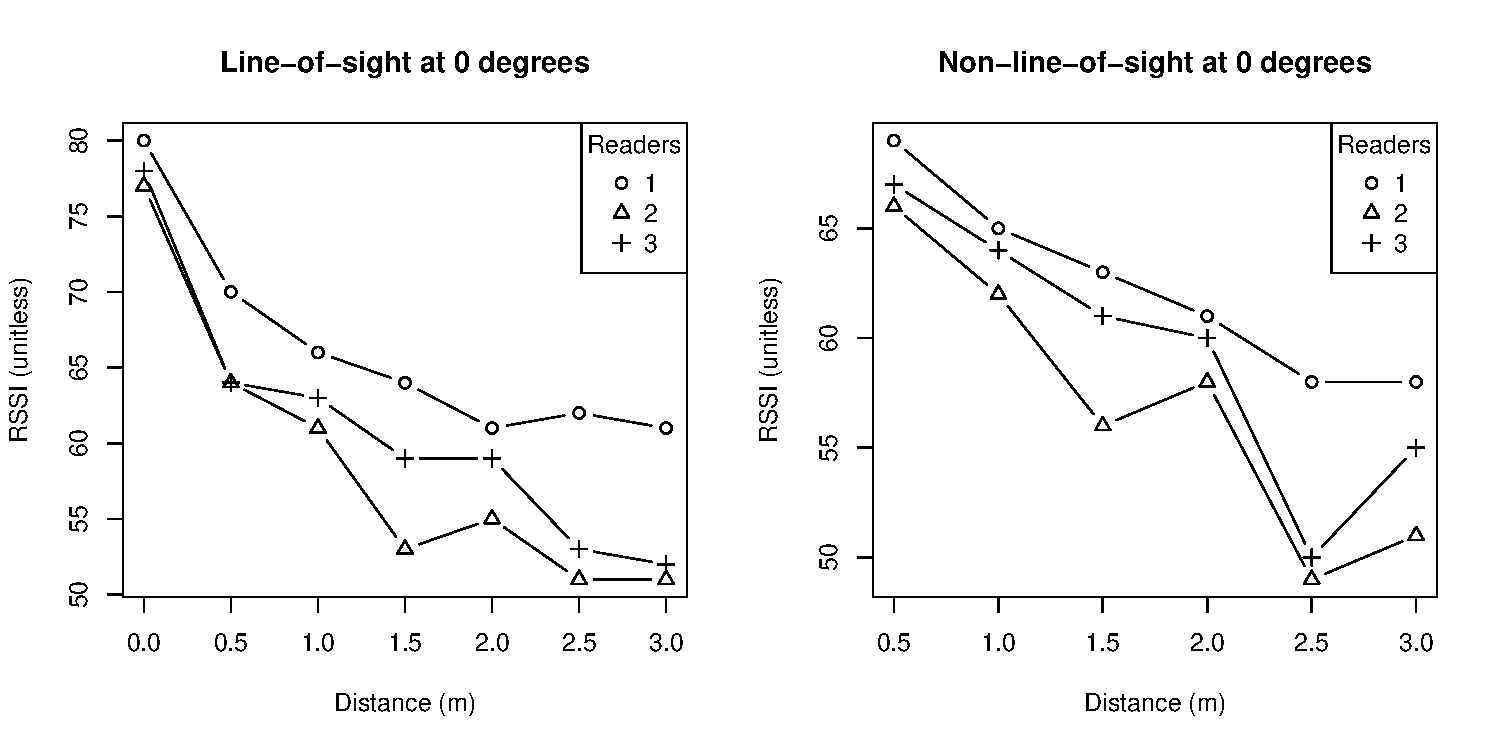
\includegraphics[width=1\textwidth]{rssi_distance_3m_0deg}
		\caption{Two plots of RSSI measurements at increasing distances with the readers at 0 degrees (antennas facing the tag). The left graph show how RSSI values change with a line-of-sight signal propagation. The right graph illustrates the same experiment but with a non-line-of-sight signal propagation (there is an obstacle between the reader and the tag).}
	\end{center}
\end{figure}
\begin{figure}
	\begin{center}
		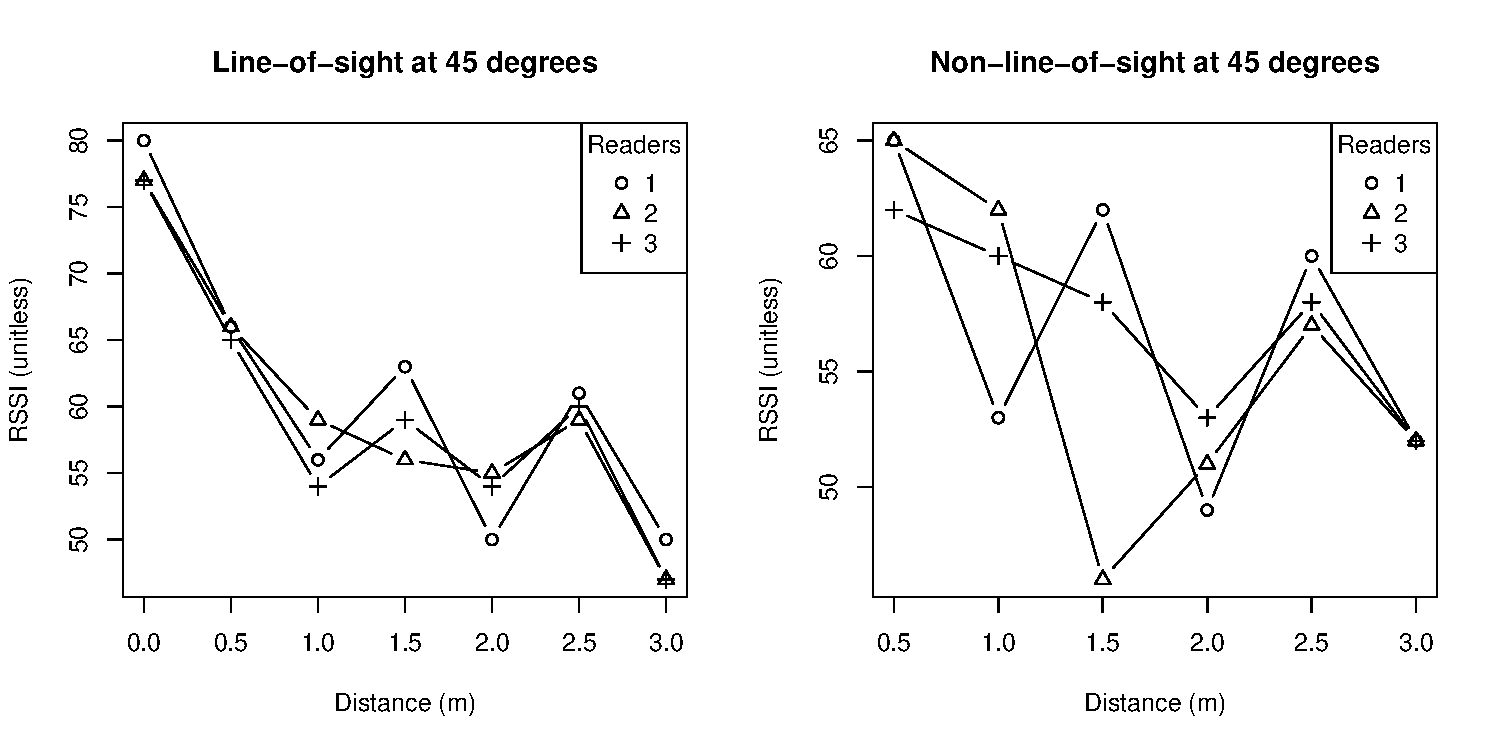
\includegraphics[width=1\textwidth]{rssi_distance_3m_45deg}
		\caption{Two plots of RSSI measurements at increasing distances with the readers at 45 degrees (antennas at an angle to the tag). The left graph show how RSSI values change with a line-of-sight signal propagation. The right graph illustrates the same experiment but with a non-line-of-sight signal propagation (there is an obstacle between the reader and the tag).}
	\end{center}
\end{figure}
\begin{figure}
	\begin{center}
		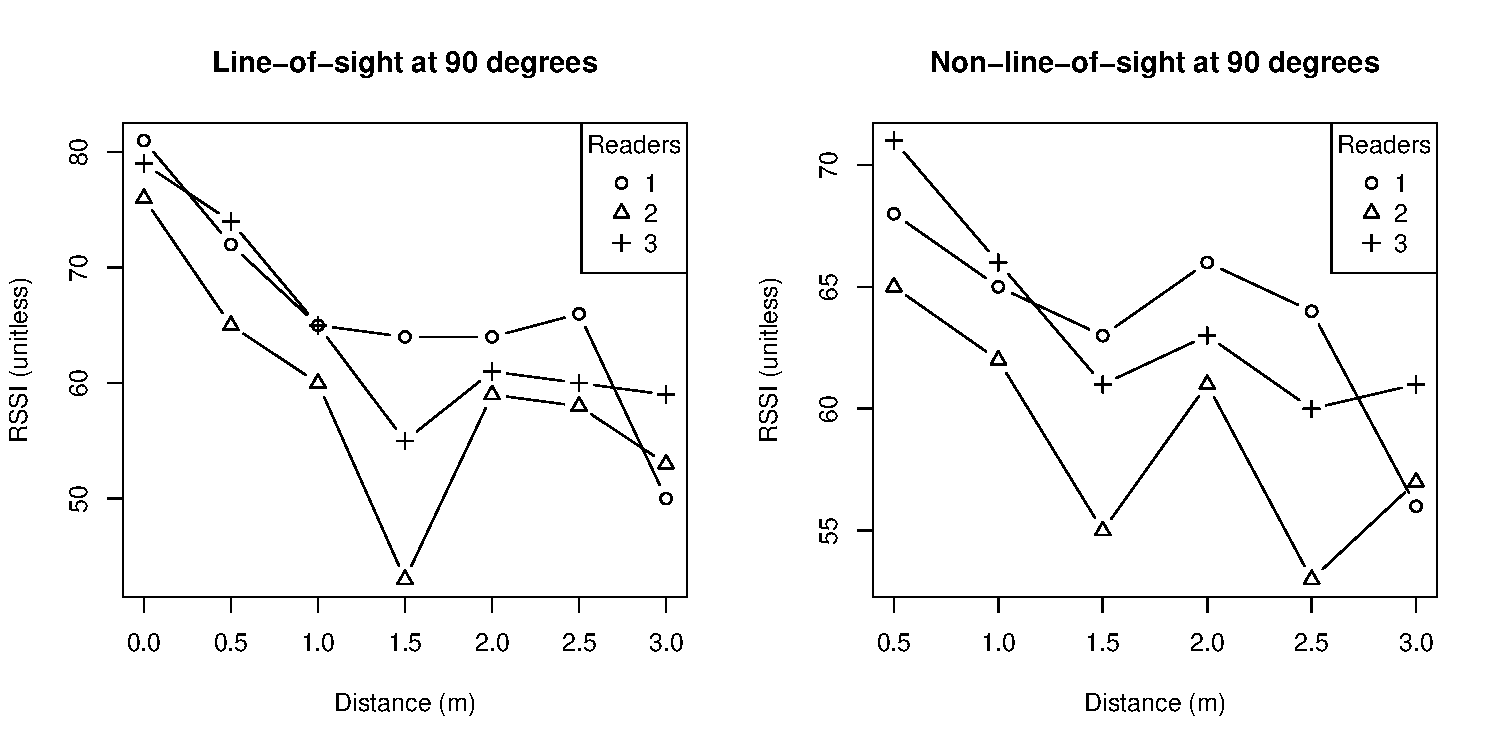
\includegraphics[width=1\textwidth]{rssi_distance_3m_90deg}
		\caption{Two plots of RSSI measurements at increasing distances with the readers at 90 degrees (antennas at an angle to the tag). The left graph show how RSSI values change with a line-of-sight signal propagation. The right graph illustrates the same experiment but with a non-line-of-sight signal propagation (there is an obstacle between the reader and the tag).}
	\end{center}
\end{figure}
\begin{figure}
	\begin{center}
		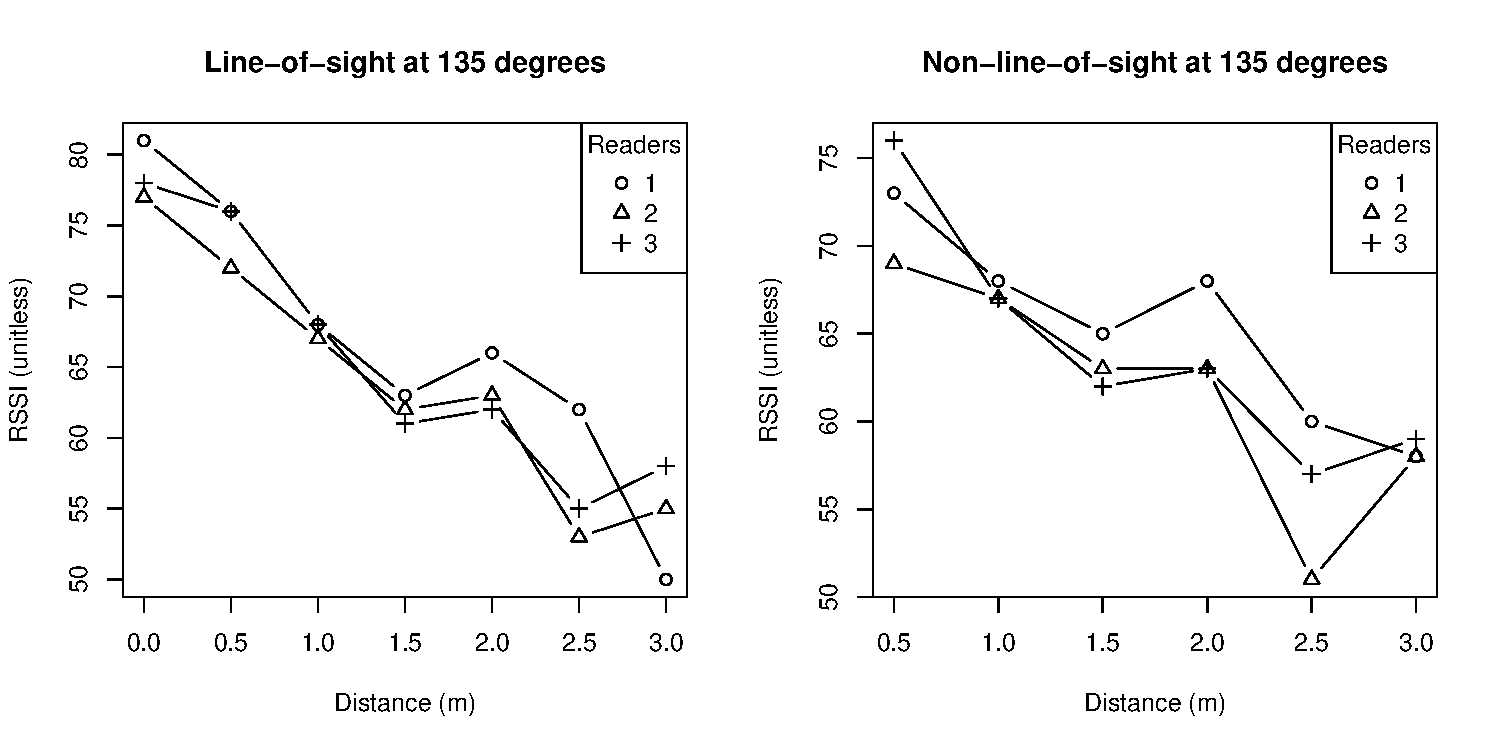
\includegraphics[width=1\textwidth]{rssi_distance_3m_135deg}
		\caption{Two plots of RSSI measurements at increasing distances with the readers at 135 degrees (antennas at an angle to the tag). The left graph show how RSSI values change with a line-of-sight signal propagation. The right graph illustrates the same experiment but with a non-line-of-sight signal propagation (there is an obstacle between the reader and the tag).}
	\end{center}
\end{figure}
\begin{figure}
	\begin{center}
		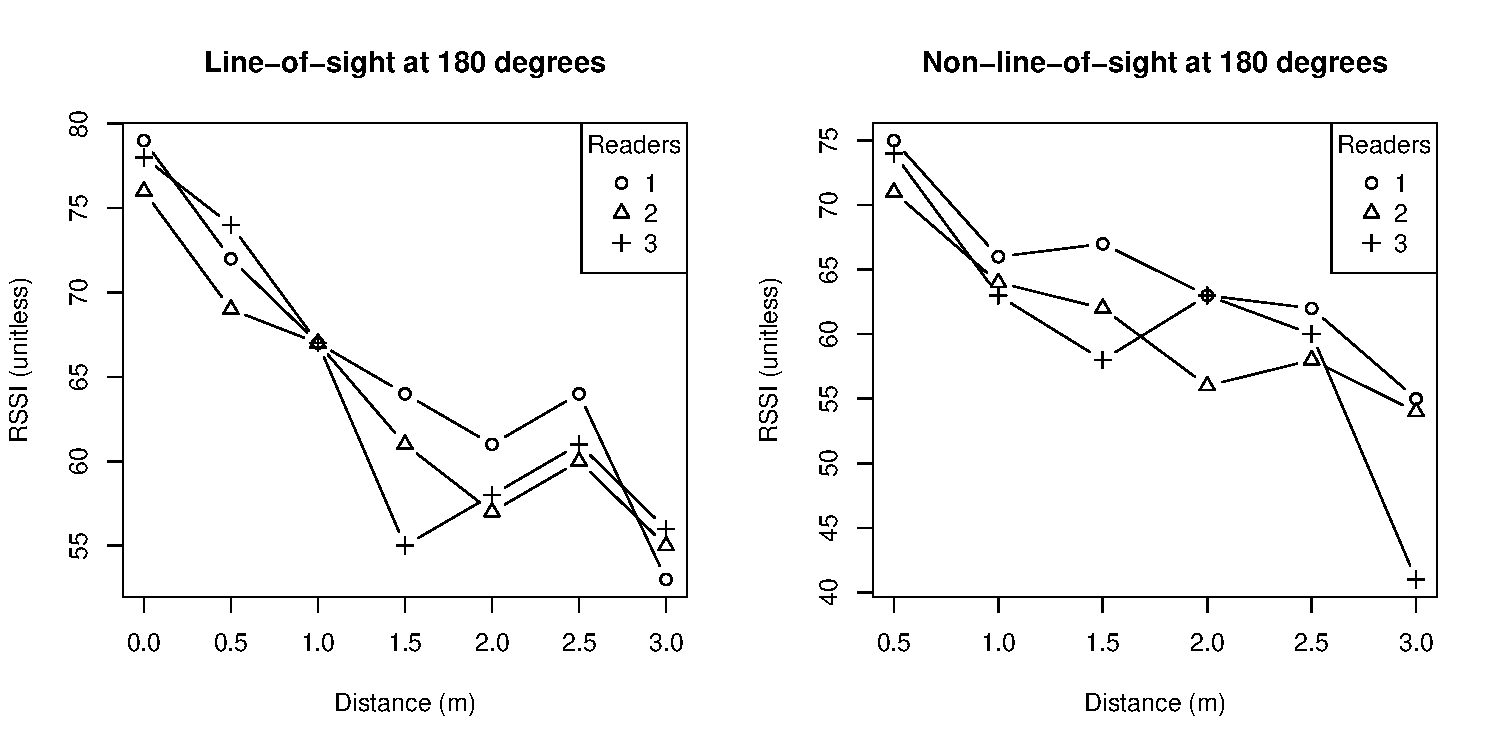
\includegraphics[width=1\textwidth]{rssi_distance_3m_180deg}
		\caption{Two plots of RSSI measurements at increasing distances with the readers at 180 degrees (antennas at an angle to the tag). The left graph show how RSSI values change with a line-of-sight signal propagation. The right graph illustrates the same experiment but with a non-line-of-sight signal propagation (there is an obstacle between the reader and the tag).}
	\end{center}
\end{figure}
\begin{figure}
	\begin{center}
		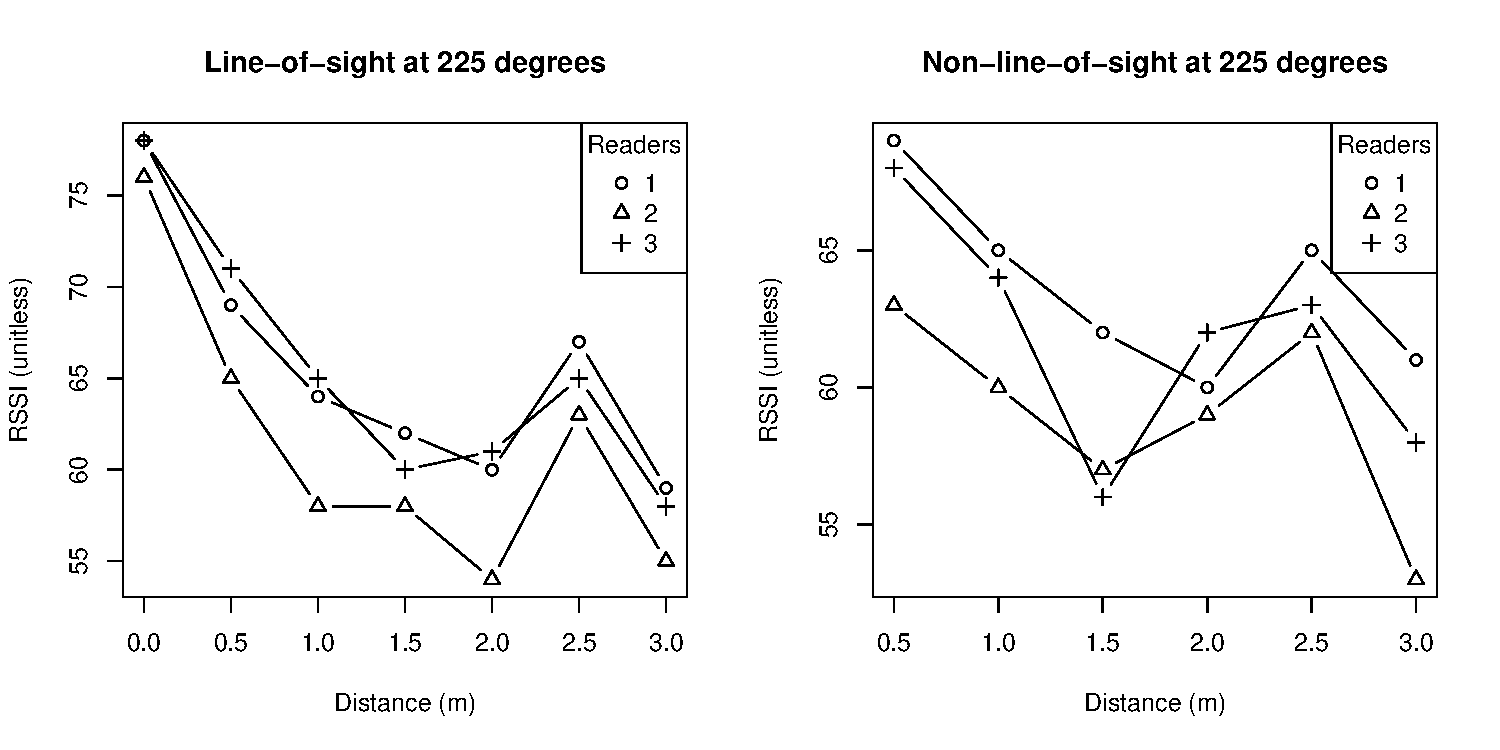
\includegraphics[width=1\textwidth]{rssi_distance_3m_225deg}
		\caption{Two plots of RSSI measurements at increasing distances with the readers at 225 degrees (antennas at an angle to the tag). The left graph show how RSSI values change with a line-of-sight signal propagation. The right graph illustrates the same experiment but with a non-line-of-sight signal propagation (there is an obstacle between the reader and the tag).}
	\end{center}
\end{figure}
\begin{figure}
	\begin{center}
		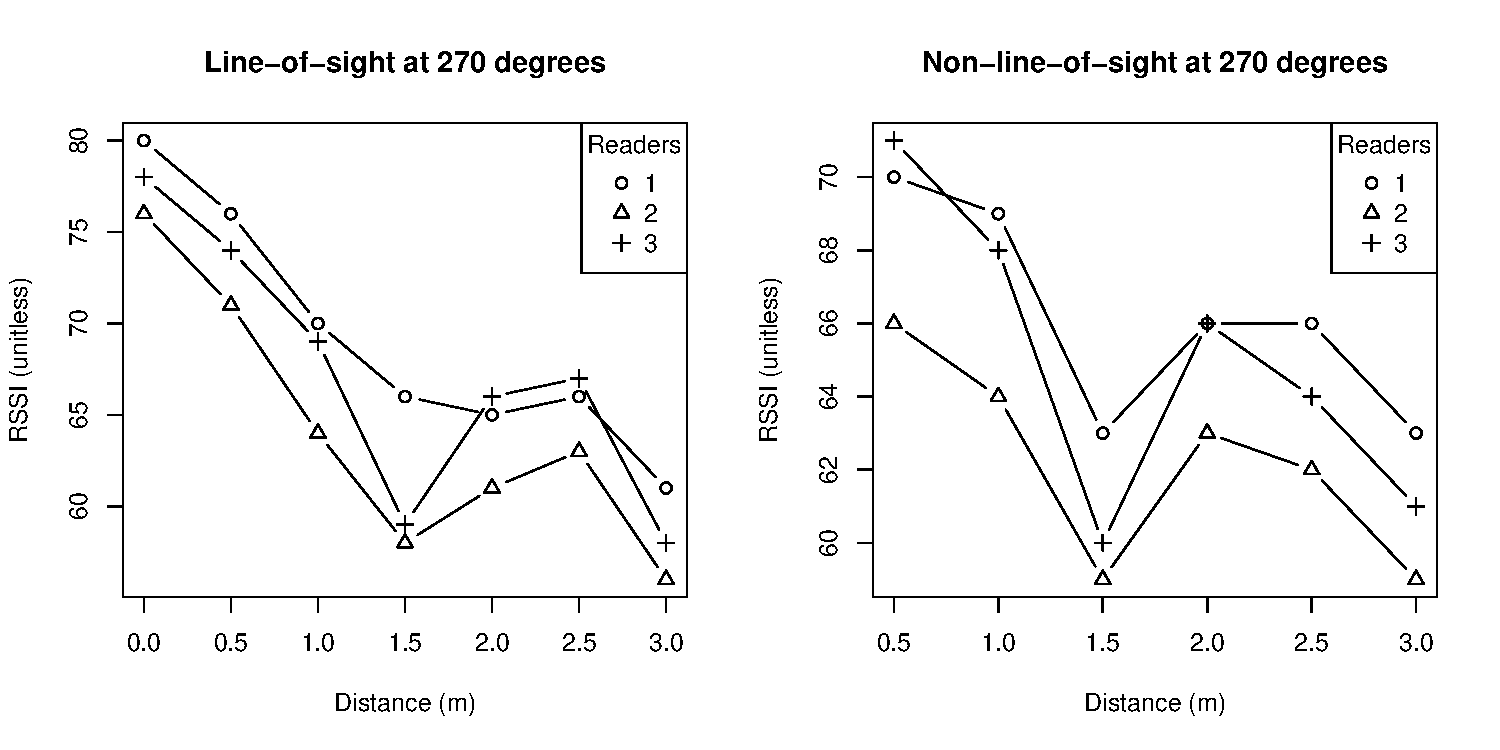
\includegraphics[width=1\textwidth]{rssi_distance_3m_270deg}
		\caption{Two plots of RSSI measurements at increasing distances with the readers at 270 degrees (antennas at an angle to the tag). The left graph show how RSSI values change with a line-of-sight signal propagation. The right graph illustrates the same experiment but with a non-line-of-sight signal propagation (there is an obstacle between the reader and the tag).}
	\end{center}
\end{figure}
\begin{figure}
	\begin{center}
		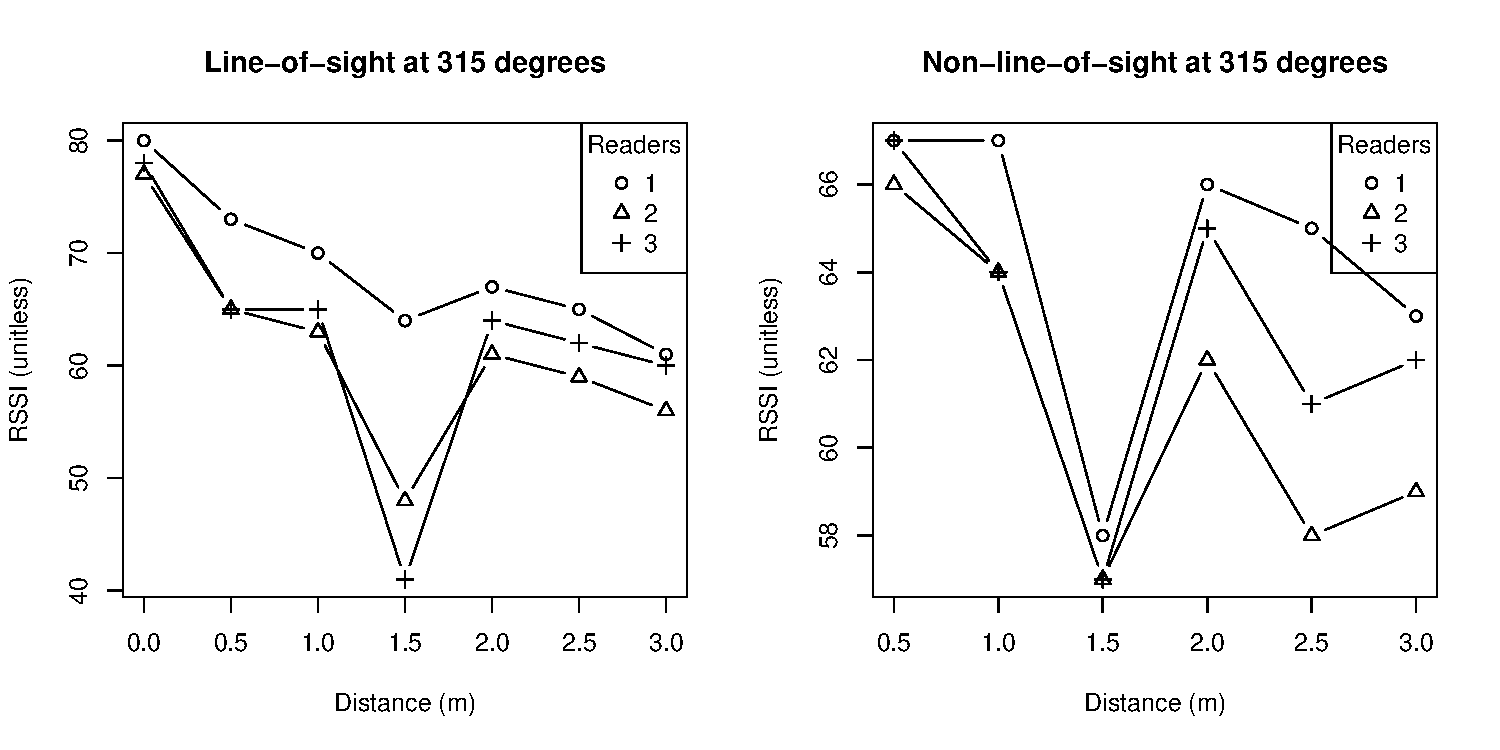
\includegraphics[width=1\textwidth]{rssi_distance_3m_315deg}
		\caption{Two plots of RSSI measurements at increasing distances with the readers at 315 degrees (antennas at an angle to the tag). The left graph show how RSSI values change with a line-of-sight signal propagation. The right graph illustrates the same experiment but with a non-line-of-sight signal propagation (there is an obstacle between the reader and the tag).}
	\end{center}
\end{figure}
\begin{figure}
	\begin{center}
		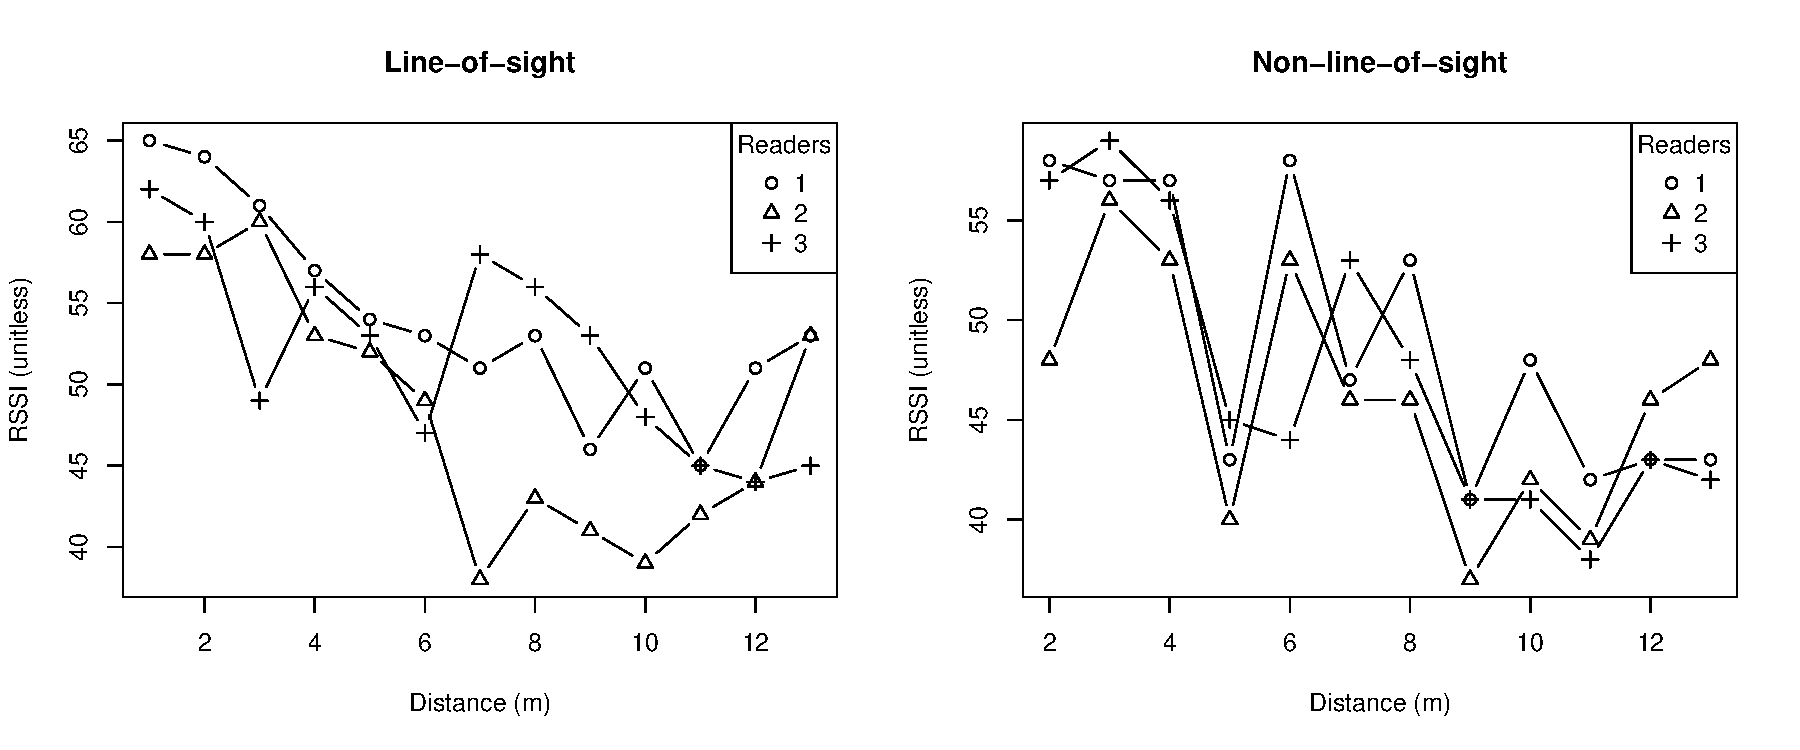
\includegraphics[width=1\textwidth]{rssi_distance_13m}
		\caption{Two plots of RSSI measurements at increasing distances with the readers facing the tag. The left graph show how RSSI values change with a line-of-sight signal propagation. The right graph illustrates the same experiment but with a non-line-of-sight signal propagation (there is an obstacle between the reader and the tag).}
	\end{center}
\end{figure}
\begin{figure}
	\begin{center}
		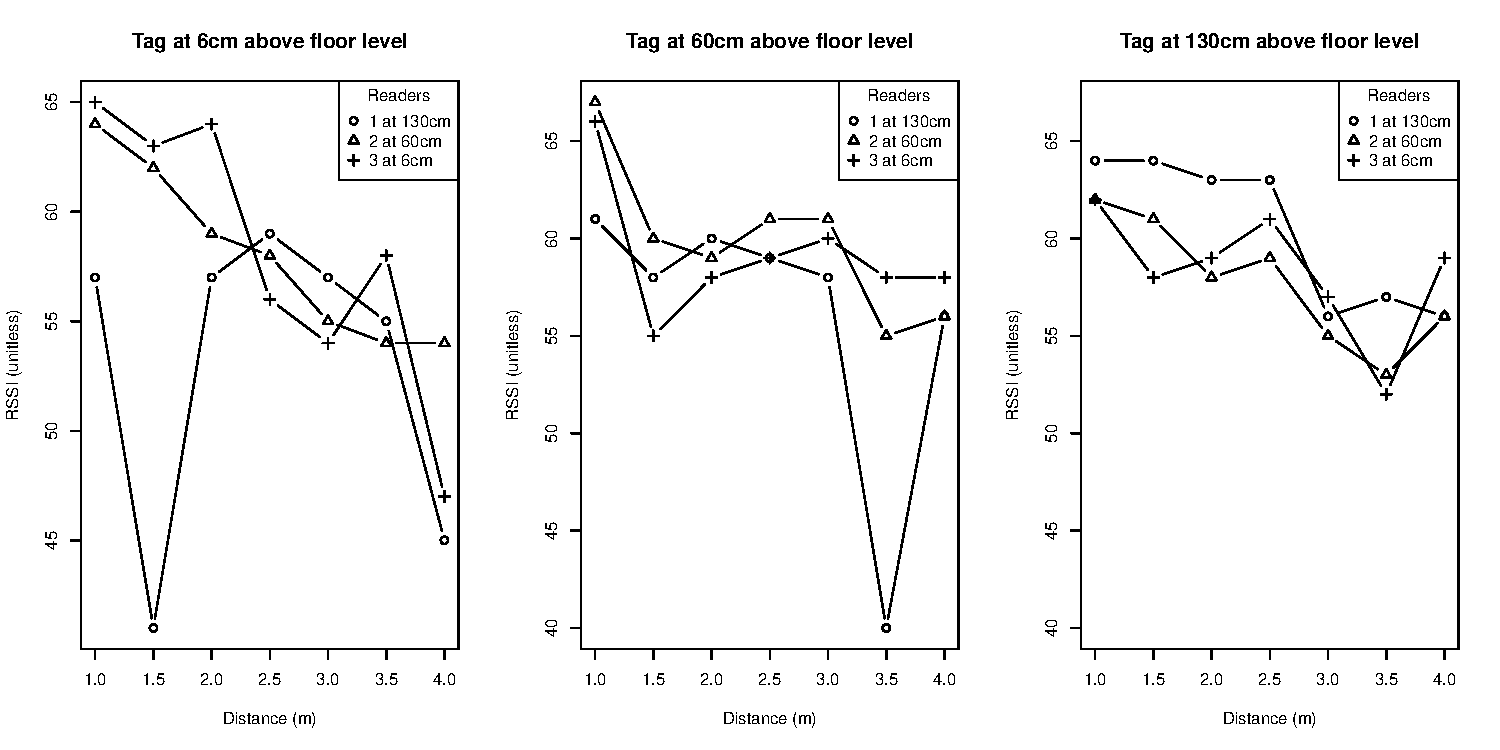
\includegraphics[width=1\textwidth]{rssi_distance_4m}
		\caption{Three plots of RSSI measurements at increasing distances with the readers at different elevation from the floor in an indoor environment. The first graph shows how RSSI measurements change as the distance grows when the tag is placed at 6cm above floor level. The second and third graph show the same experiment but the tag is at 60cm and 130cm above the floor level.}
	\end{center}
\end{figure}
\begin{figure}
	\begin{center}
		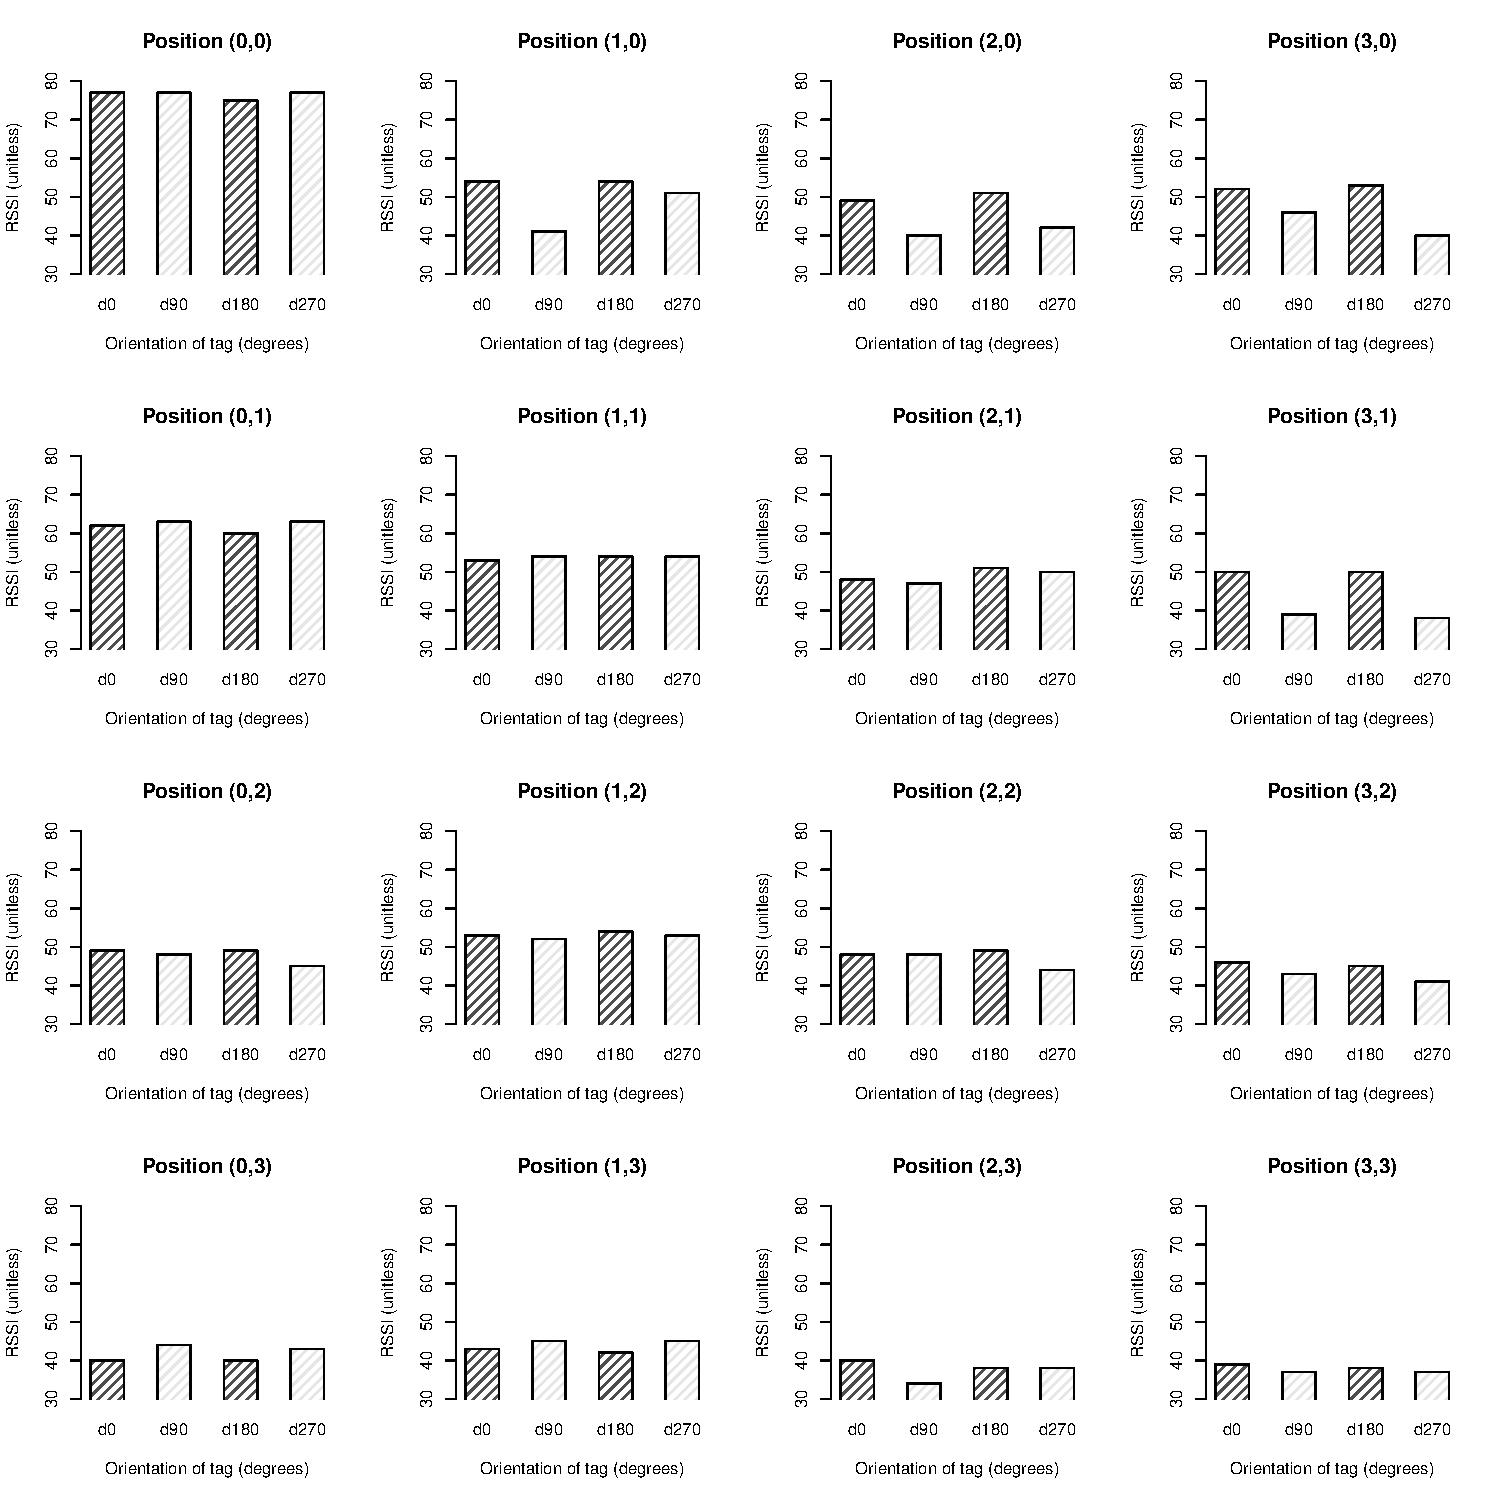
\includegraphics[width=1\textwidth]{rssi_distance_grid_r1}
		\caption{Sixteen plots are organised into a four by four grid. Each plot represents the RSSI measurements of the \textbf{first} reader when the tag is placed at different positions on the x and y axes of the grid. The positions of the tag are all measured in meters. Every four bars in each plot show the RSSI readings when the tag is facing right (0\textdegree), up(90\textdegree), left (180\textdegree), and down (270\textdegree).}
	\end{center}
\end{figure}
\begin{figure}
	\begin{center}
		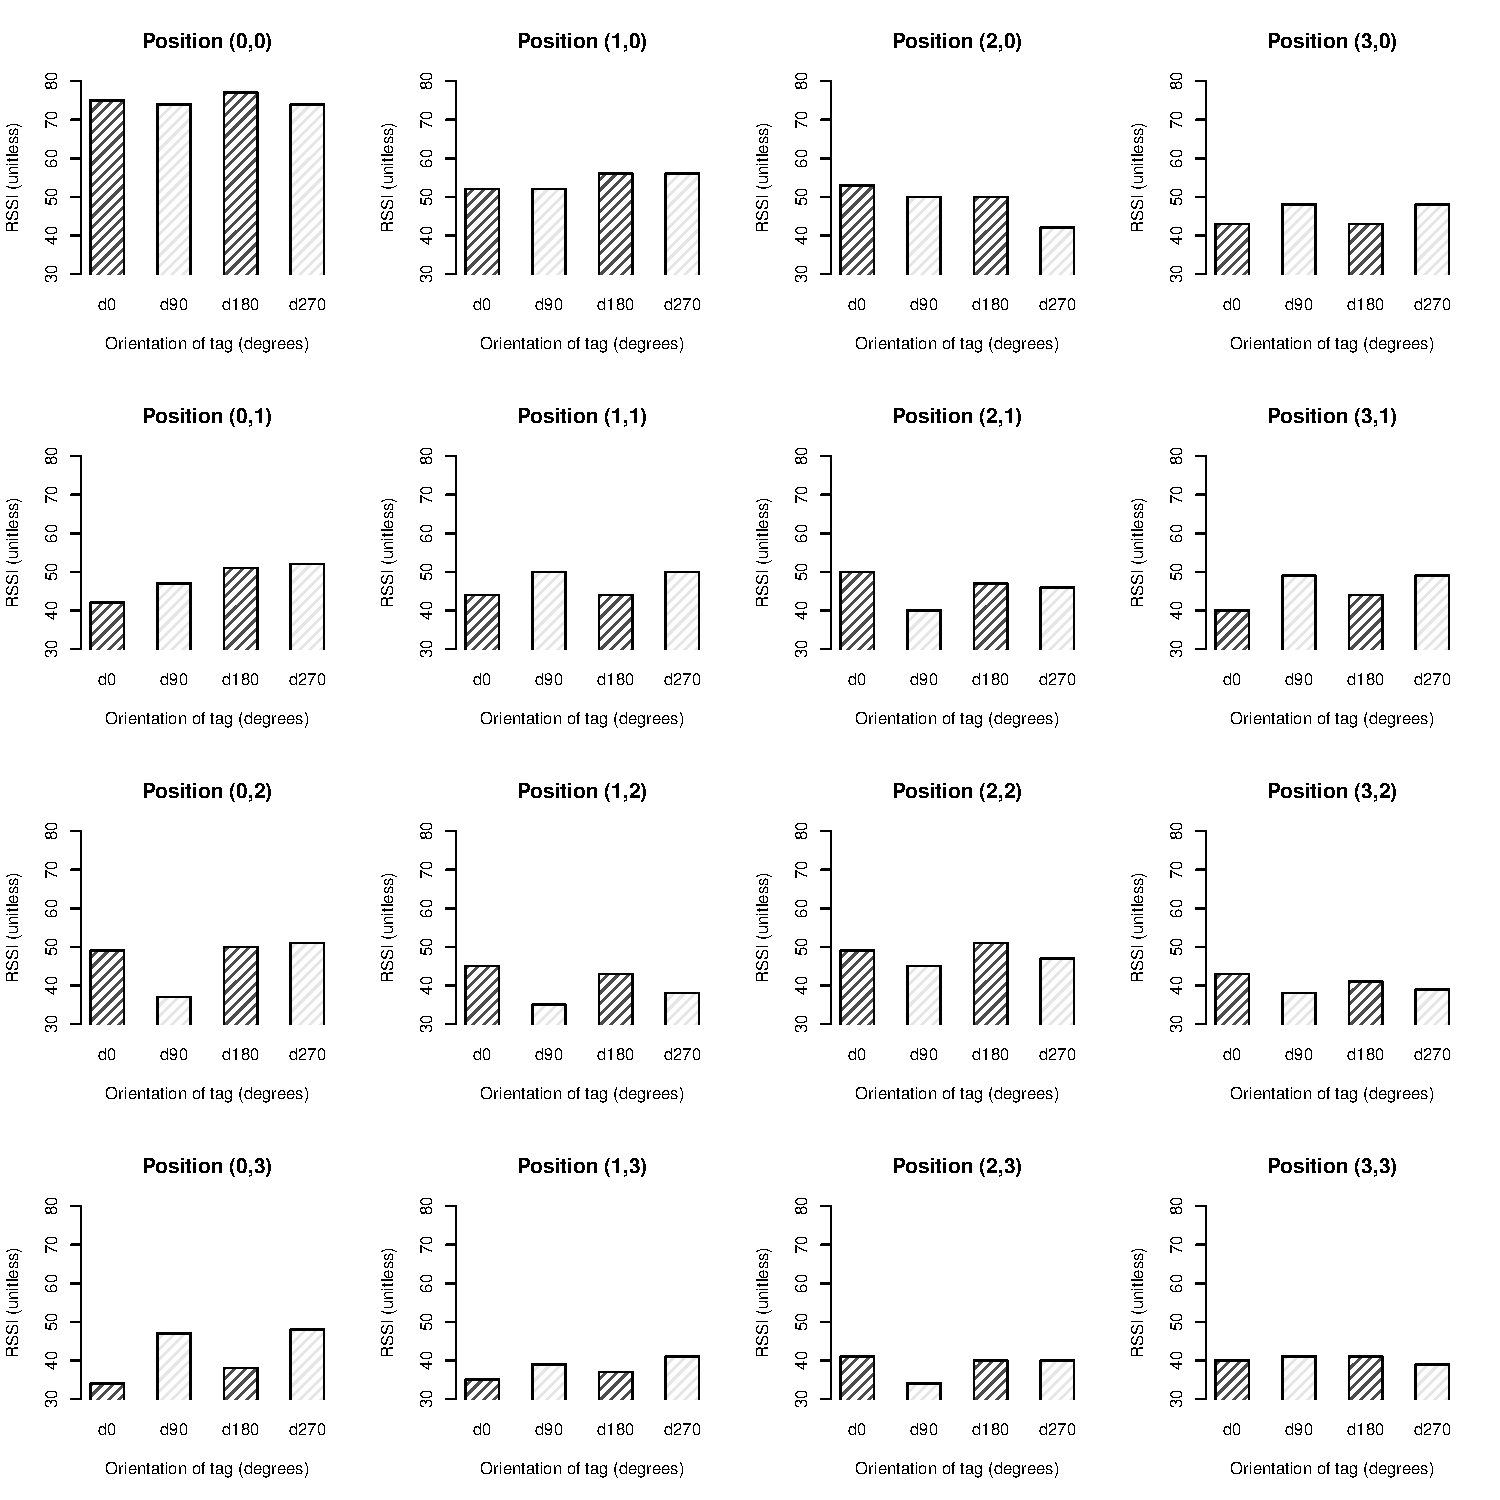
\includegraphics[width=1\textwidth]{rssi_distance_grid_r2}
		\caption{Sixteen plots are organised into a four by four grid. Each plot represents the RSSI measurements of the \textbf{second} reader when the tag is placed at different positions on the x and y axes of the grid. The positions of the tag are all measured in meters. Every four bars in each plot show the RSSI readings when the tag is facing right (0\textdegree), up(90\textdegree), left (180\textdegree), and down (270\textdegree).}
	\end{center}
\end{figure}
\begin{figure}
	\begin{center}
		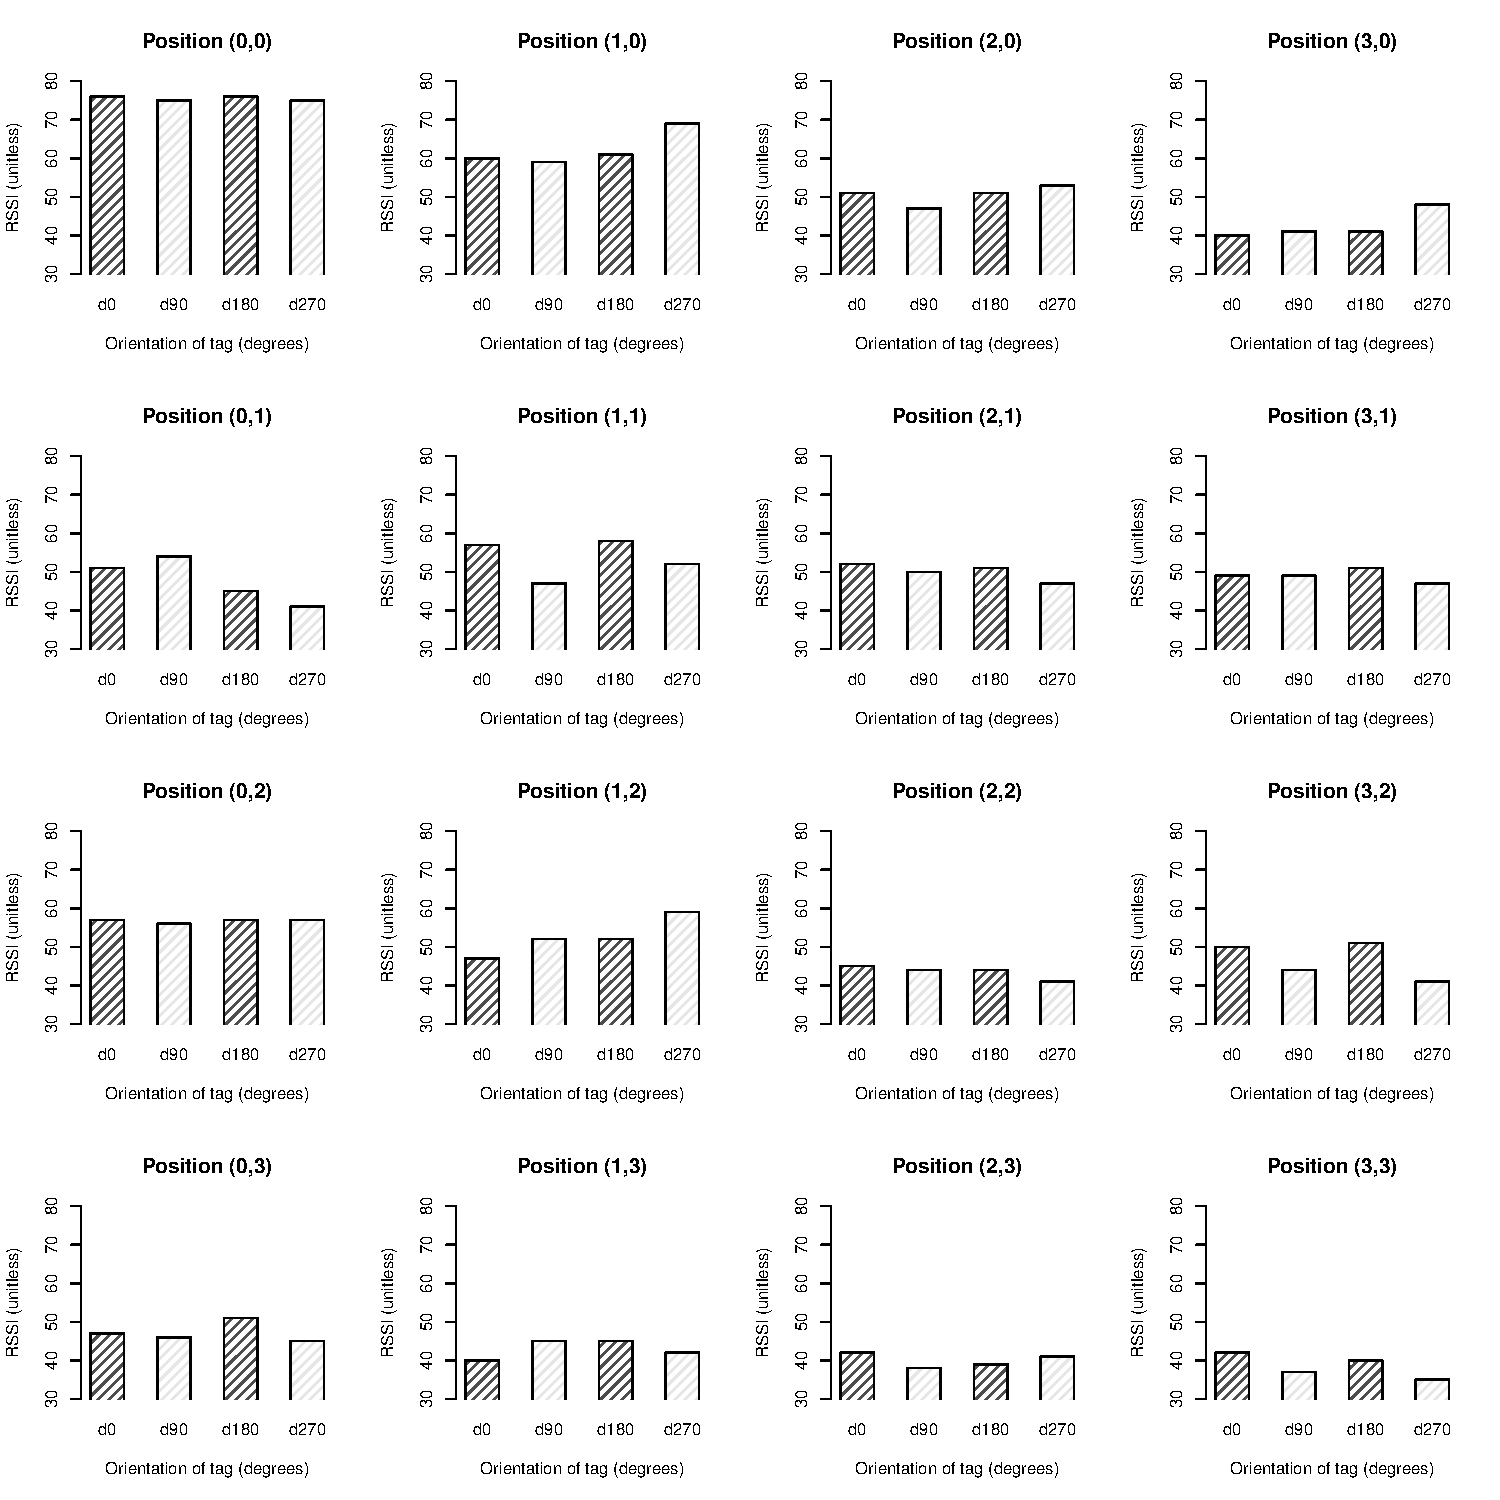
\includegraphics[width=1\textwidth]{rssi_distance_grid_r3}
		\caption{Sixteen plots are organised into a four by four grid. Each plot represents the RSSI measurements of the \textbf{third} reader when the tag is placed at different positions on the x and y axes of the grid. The positions of the tag are all measured in meters. Every four bars in each plot show the RSSI readings when the tag is facing right (0\textdegree), up(90\textdegree), left (180\textdegree), and down (270\textdegree).}
	\end{center}
\end{figure}
\begin{figure}
	\begin{center}
		
\includegraphics[width=1\textwidth]{error_distance_grid}
		\caption{Sixteen plots are organised into a four by four grid. The readers are placed at positions (0,0), (0,3), and (3,0). Each plot represents the error in meters between measured and estimated location when the tag is placed at different positions on the grid. Each plot consists of four ellipses that illustrate the x and y error when the tag is facing right (0\textdegree), up(90\textdegree), left (180\textdegree), and down (270\textdegree). The colours of the ellipses are red, green, blue, and black, respectively.}
	\end{center}
\end{figure}

\section{July 16, Tuesday}

\begin{itemize}
	\item Created a box plot using the errors of the last experiment.
	\item Wrote captions for every plot I created.
\end{itemize}

\begin{figure}
	\begin{center}
		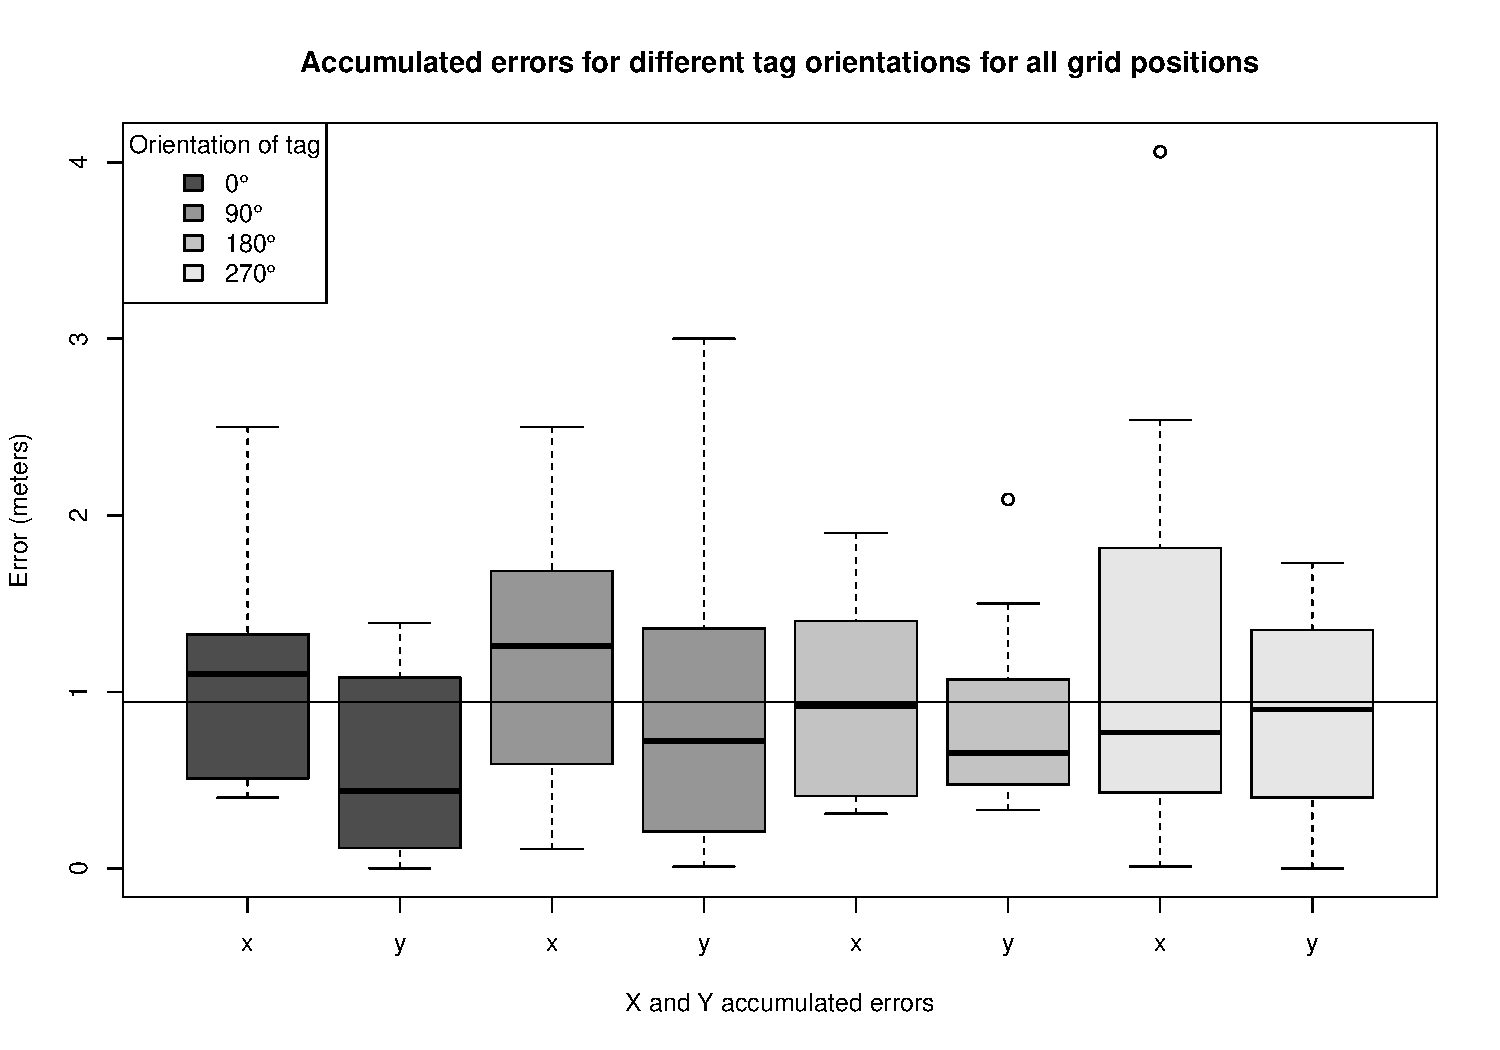
\includegraphics[width=1\textwidth]{error_boxplot}
		\caption{A box plot showing errors between measured and estimated locations. The boxes are organised in four groups. Each group consists of errors in the x and y axes for a particular orientation of the tag. The horizontal line across the plot is the mean of all errors regardless of the tag orientation.}
	\end{center}
\end{figure}

\newpage
\bibliographystyle{apalike}
\bibliography{../library}

\end{document}
